\documentclass{beamer}

\usepackage{graphics}
\usepackage{graphicx}
\usepackage{hyperref}
\usepackage[latin1]{inputenc}

\title[Introdution to SOFA]{An Introduction to Sofa}
\author[Faure]{%
  Fran�ois~Faure\inst{1} }
\institute[Univ. Grenoble]{
  \inst{1}%
  University Joseph Fourier, Grenoble\\
  INRIA - Evasion
  }
\date[September 2007]{September 11th 2007}
\subject{Computational Sciences}


\begin{document}

  \frame
  {
    \titlepage
  }

\section{Overview}

\begin{frame}
 \frametitle{Main Features}
\begin{itemize}
 \item High modularity using a scene graph
 \item Multiple models of the same object can be synchronized using mappings
\end{itemize}

\end{frame}

\begin{frame}
 \frametitle{Data structure}
Scene graph with three levels of hierarchy
\begin{itemize}
 \item Nodes contains Nodes and Components.
 \item Components are leaves of the scene graph. They implement algorithms. They contain DataFields.
\item DataFields contain raw data (positions, masses, ...)
\end{itemize}
Example: A mass-spring string and a rigid body
\begin{figure}
\newcommand{\heigh}{25mm}
\begin{tabular}{ccc}
\begin{tabular}{c}
 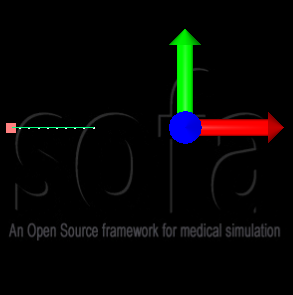
\includegraphics[height=\heigh]{mixed1.png} \\ the objects: \\ one string\\on rigid
\end{tabular}
&
\begin{tabular}{c}
 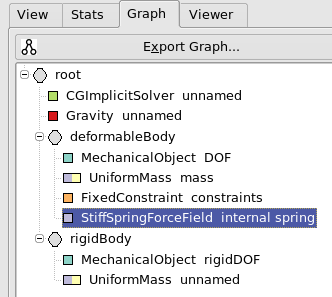
\includegraphics[height=\heigh]{mixed3.png} \\ scene graph: \\ 3 nodes\\8 components 
\end{tabular}
&
\begin{tabular}{c}
 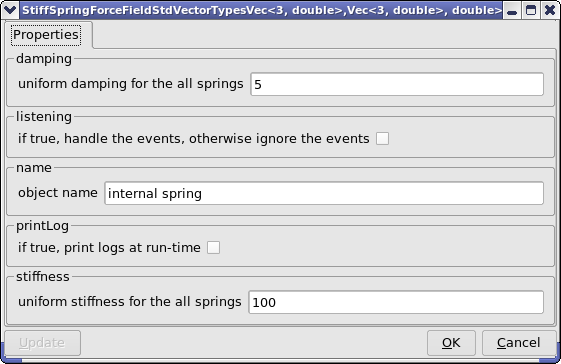
\includegraphics[height=\heigh]{mixed4.png} \\ the datafields of a\\ selected component \\
\end{tabular}
\end{tabular}
\end{figure}

\end{frame}


\begin{frame}
\frametitle{Why using scene graphs}
\begin{itemize}
 \item standard graphics tool (VRML, Java3D, ...)
 \item dynamically add or remove objects in the scene
 \item replacing a component while leaving the others unchanged
 \item I/O file format
\end{itemize}
\end{frame}

\begin{frame}
 \frametitle{Multiple models of a given object}
\begin{columns}
 \column{0.5\linewidth}
\begin{itemize}
 \item different geometries for different purposes
 \item one master geometry (mechanical behavior) contains the independent degrees of freedom (dof)
 \item implemented as a node hierarchy
 \item non-independent dofs updated using \emph{mappings}
\end{itemize}

 \column{0.5\linewidth}
\begin{figure}
 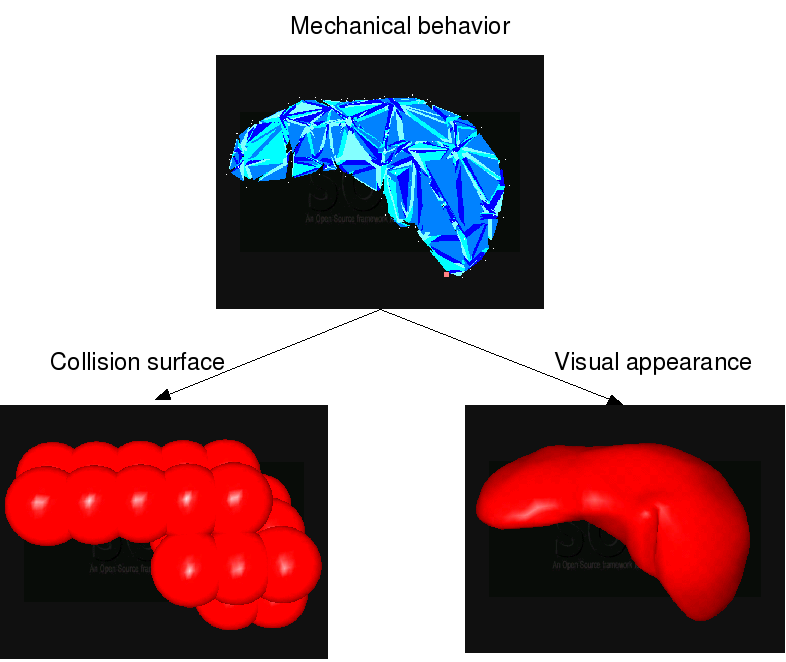
\includegraphics[width=\linewidth]{slides-fig-multimodal.png}
\end{figure}

\end{columns}
\end{frame}



\begin{frame}
 \frametitle{Example of mapping}
\begin{columns}
 \column{0.6\linewidth}
\begin{itemize}
 \item 4 mechanical control points
 \item one finite element (tetrahedron)
 \item hundreds of vertices in the visual model, all totally defined by the mechanical control points
\end{itemize}
\begin{tabular}{c}
 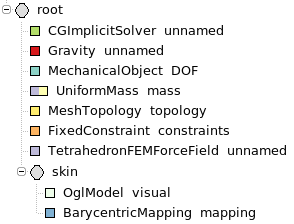
\includegraphics[width=\linewidth]{mixed7.png}
\end{tabular}

 \column{0.4\linewidth}
\begin{figure}
\begin{tabular}{c}
 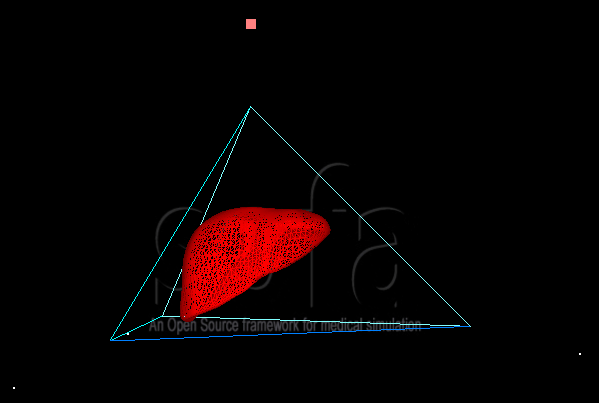
\includegraphics[width=\linewidth]{mixed5.png}\\
 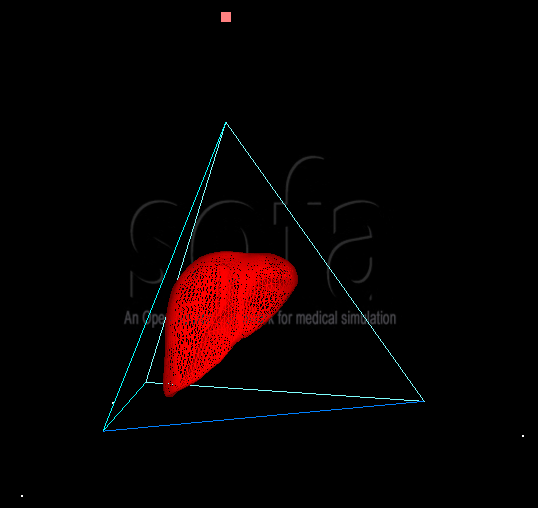
\includegraphics[width=\linewidth]{mixed6.png}
\end{tabular}
\end{figure}

\end{columns}
\end{frame}

\begin{frame}
 \frametitle{A more complete picture of the scene graph}
\begin{itemize}
 \item The graph displayed in the GUI shows only the hierarchy:\\ 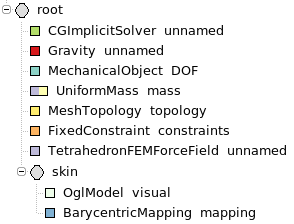
\includegraphics[width=0.5\linewidth]{mixed7.png}
 \item Additional pointers appear in the graph exported and displayed using graphviz: 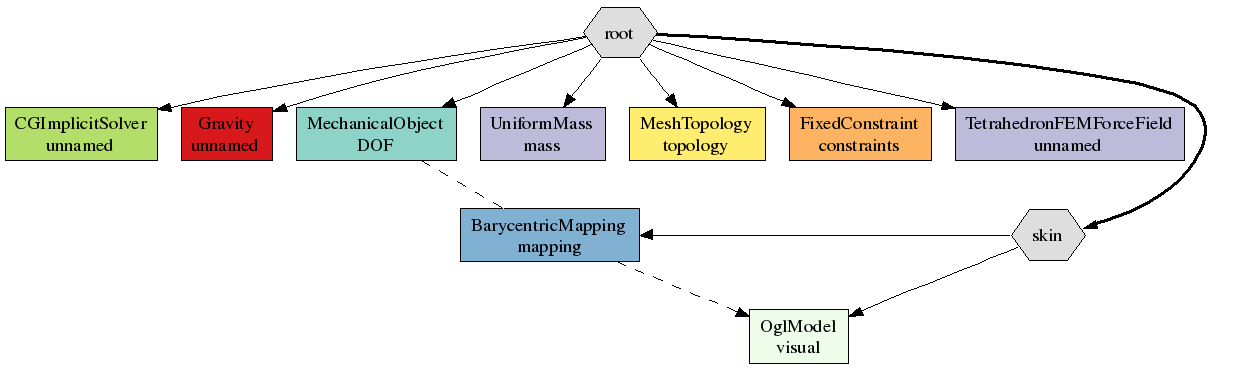
\includegraphics[width=\linewidth]{mixed8.png}
\end{itemize}
\end{frame}


\begin{frame}
 \frametitle{Interacting bodies}
\begin{itemize}
 \item We attach a point to the rigid body using a mapping
 \item We insert a spring between this point and the string
\end{itemize}
\begin{figure}
 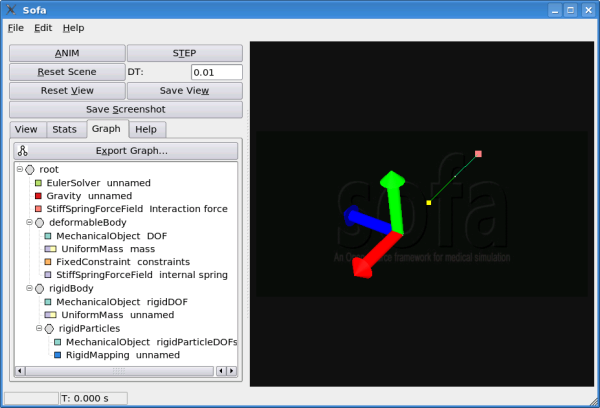
\includegraphics[width=0.8\linewidth]{mixedPendulum.png}
\end{figure}
\end{frame}

\begin{frame}
 \frametitle{Interacting bodies}
Complete graph with pointers
\begin{itemize}
 \item We attach a point to the rigid body using a mapping
 \item We insert a spring between this point and the string
\end{itemize}
\begin{figure}
 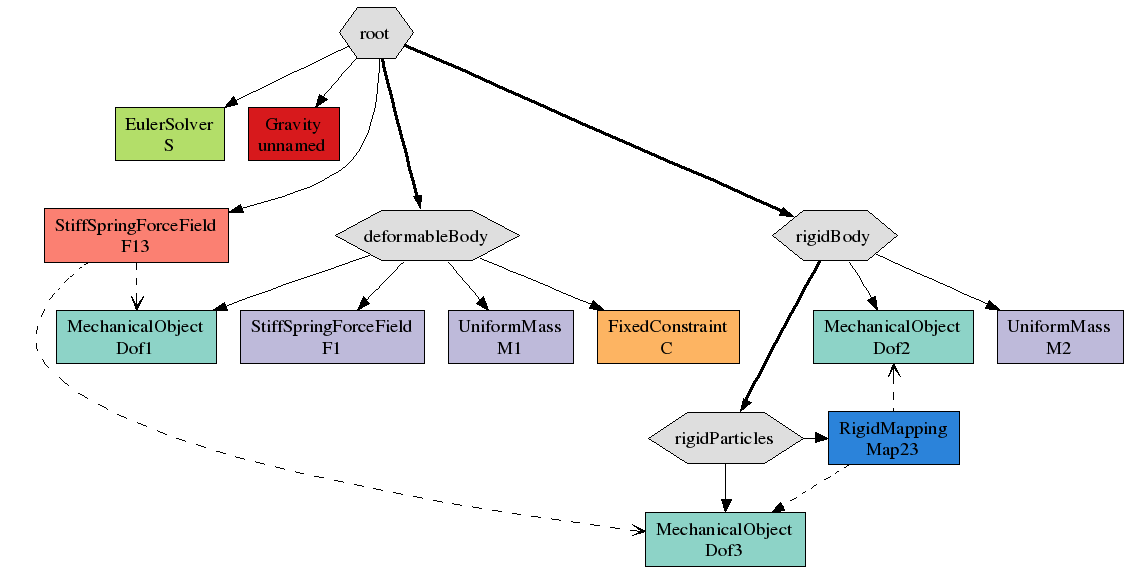
\includegraphics[width=0.99\linewidth]{mixedPendulum-graph.png}
\end{figure}
\end{frame}


\begin{frame}
\frametitle{Interacting bodies}
Without interaction force
\begin{figure}
\begin{tabular}{c}
 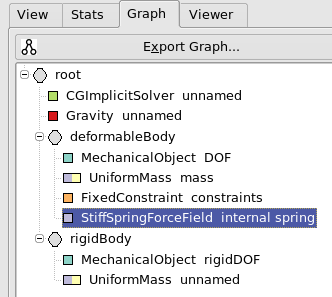
\includegraphics[height=3cm]{mixed3.png} \\ scene graph
\end{tabular}
\begin{tabular}{c}
 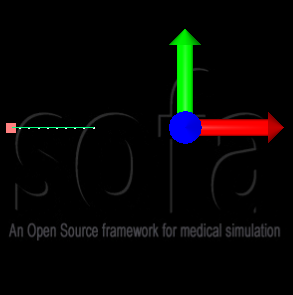
\includegraphics[height=3cm]{mixed1.png} \\ t=0
\end{tabular}
\begin{tabular}{c}
 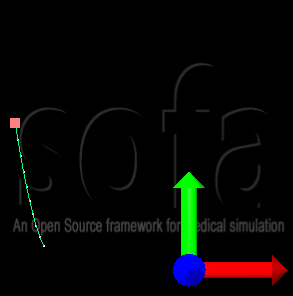
\includegraphics[height=3cm]{mixed2.png} \\ t = ...
\end{tabular}
\end{figure}
\end{frame}


\begin{frame}
\frametitle{Interacting bodies}
With interaction force
\begin{figure}
\begin{tabular}{c}
 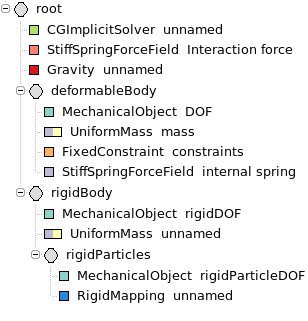
\includegraphics[height=3.7cm]{mixed11.png} \\ scene graph
\end{tabular}
\begin{tabular}{c}
 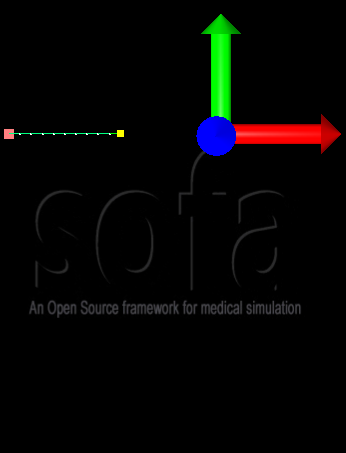
\includegraphics[height=3.7cm]{mixed9.png} \\ t=0
\end{tabular}
\begin{tabular}{c}
 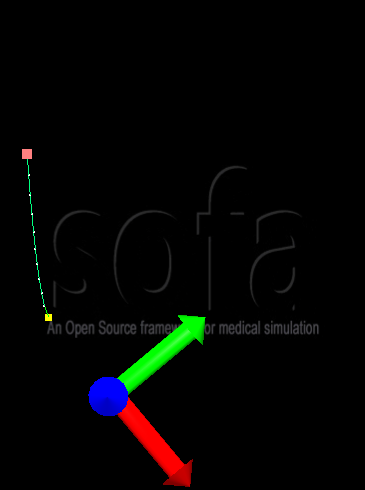
\includegraphics[height=3.9cm]{mixed10.png} \\  t = ...
\end{tabular}
\end{figure}
\end{frame}






\begin{frame}
 \frametitle{Data processing}
Sofa Actions:
\begin{itemize}
 \item The scene graph is recursively traversed top-down and bottom-up
 \item Callbacks are applied to components of certain classes
 \item Used for all operations: physical computations, vector operations, collision detection,...
 \item Example: accumulate forces
   \begin{itemize}
    \item top-down: masses and force fields accumulate force
    \item bottom-up: mappings dispatch forces to their parents
   \end{itemize}

\end{itemize}

\end{frame}






\end{document}
